%%% ---------- How to make headlines and sections ---------- %%%
\section{This is a section} \label{sec:thisSection}
\subsection{This is a subsection}
Let us refer to section \ref{sec:thisSection}.

%%% How to write bold, italics %%%
This text is \textbf{bold}.
This text is \textit{italics}.

%%% ---------- Insert page break ---------- %%%
%%\newpage
%%Here is some text on the next page

%%% ---------- This is how you refer to a figure in the text ---------- %%%
Here is something that I illustrate in figure \ref{fig:wavelength}.

%%% ---------- This is how you insert a single picture ---------- %%%
\begin{figure}[htbp]
\centering
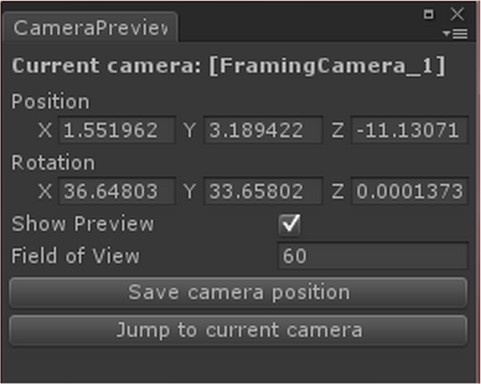
\includegraphics[width=0.50\textwidth]{Pics/Dummy}
\caption{Image caption text goes here bla bla bla bla}
\label{fig:wavelength}
\end{figure}

%%% ---------- This is how you insert multiple pictures ---------- %%%
\begin{figure}[htbp] \centering
\begin{minipage}[b]{0.45\textwidth} \centering
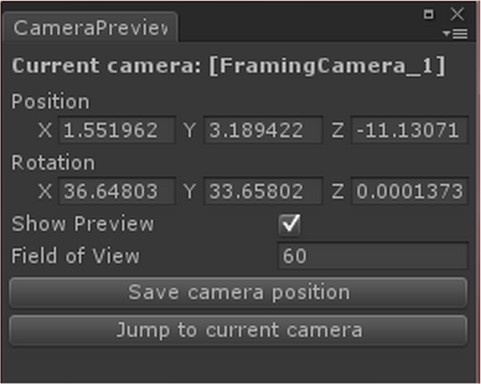
\includegraphics[width=0.60\textwidth]{Pics/Dummy} % Venstre billede
\end{minipage} \hfill
\begin{minipage}[b]{0.45\textwidth} \centering
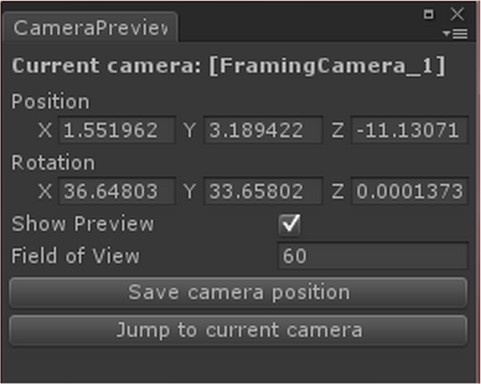
\includegraphics[width=0.60\textwidth]{Pics/Dummy} % Højre billede
\end{minipage} \\ % Captions og labels
\begin{minipage}[t]{0.45\textwidth}
\caption{Caption text for left picture.} % Venstre caption og label
\label{fig:cap1}
\end{minipage} \hfill
\begin{minipage}[t]{0.45\textwidth}
\caption{Caption text for right picture} % Højre caption og label
\label{fig:cap2}
\end{minipage}
\end{figure}

%%% ---------- This is how to make a source reference ---------- %%%
According to bla bla \cite{haigh-hutchinson_real-time_2009} %% passive source
at cite flere: \cite{haigh-hutchinson_real-time_2009, haigh-hutchinson_real-time_2009, haigh-hutchinson_real-time_2009}


%%% ---------- This is how to make bullet points ---------- %%%
\begin{itemize}
\item \textbf{Wavelenght} - Measured in meters from wave top to wave top and denoted as $\lambda$.
\item \textbf{Frequency} - Measured in oscillations per second, Hz, denoted $f$.
\item \textbf{Energy} - Measured in electronvolts, eV, denoted $E$.
\end{itemize}

%%% ---------- This is how to do math stuff ---------- %%%
To derive the wavelength or the frequency, formula \ref{eq:wavelenght} is applied:
\begin{align}
\centering 
\lambda = \frac{C}{f}
\label{eq:wavelenght} 
\end{align}
where {$C$} is the speed of light.



%%% This is how to make footnotes %%%
Hello, I need a footnote \footnote[0]{You can read me, no?}.

%%% This is how to insert a table %%%
\begin{table}[htbp]
\centering
\begin{tabular}{|l|c|c|}
\hline
& Personer
& Totalpris \\\hline
Lasagne
& 4
& 160
\\\hline
Flødekartofler
& 6
& 210
\\\hline
\end{tabular}
\caption{Valg af mad.}
\label{tab:mums}
\end{table}